\documentclass[10pt,twocolumn]{extarticle}
\usepackage[a4paper,margin=1.5cm,columnsep=0.7cm]{geometry}
\usepackage{amsmath,amssymb}
\usepackage{graphicx}
\usepackage{enumitem}
\usepackage{booktabs}
\usepackage{array}
\usepackage{tabularx}
\usepackage[T1]{fontenc}

\setlength{\parindent}{0pt}
\setlength{\parskip}{4pt}
\renewcommand{\arraystretch}{1.15}

\newenvironment{qoptions}{\begin{itemize}[leftmargin=1.8em,itemsep=2pt,topsep=2pt,label={}]}{\end{itemize}}
\newcommand{\opt}[2]{\item[({#1})] {#2}}

\newcommand{\sectionhdr}[1]{\par\vspace{4pt}\noindent\textbf{\large #1}\par\vspace{2pt}}
\newcommand{\subsectionhdr}[1]{\par\vspace{3pt}\noindent\textbf{#1}\par\vspace{2pt}}

\pagestyle{empty}

\begin{document}
\twocolumn[
\begin{center}
{\LARGE\bfseries JEE (Main+Advanced) Score-II --- Test 36 (07 Feb 2025)}
\end{center}
\vspace{6pt}
]

\sectionhdr{PART-1: PHYSICS}
\subsectionhdr{Section-I (i): Single Correct}

\textbf{1.} In a YDSE both slits produce equal intensities on the screen. A 100\% transparent thin glass film is placed in front of one of the slits. Now the intensity of the geometrical centre of system on the screen becomes 75\% of the previous intensity. The wavelength of the light in vacuum is 6000\AA\ and $\mu_{\text{glass}}=1.5$. The thickness of the film cannot be:-

\begin{qoptions}
\opt{A}{$0.2\ \mu$m}
\opt{B}{$1.0\ \mu$m}
\opt{C}{$1.4\ \mu$m}
\opt{D}{$1.6\ \mu$m}
\end{qoptions}

\textbf{2.} A coil having N turns is wound tightly in the form of a spiral with inner and outer radii a and b respectively. When a current I passes through the coil, the magnetic field at the centre is

\begin{qoptions}
\opt{A}{$\dfrac{\mu_0NI}b$}
\opt{B}{$\dfrac{2\mu_0NI}a$}
\opt{C}{$\dfrac{\mu_0NI}{2(b-a)}\ln\dfrac ba$}
\opt{D}{$\dfrac{\mu_0IN}{2(b-a)}\ln\dfrac ba$}
\end{qoptions}

\textbf{3.} When an electron accelerated by potential difference U is bombarded on a specific metal the emitted X-ray spectrum obtained is shown in adjoining graph. If the potential difference is reduced to U/3, the correct spectrum is:-

\begin{figure*}[t]
\centering

\includegraphics[width=0.42\textwidth]{Score-II - Test 36 (07 Feb 2025)-img/p1phy_q3_stem.png}\\[6pt]
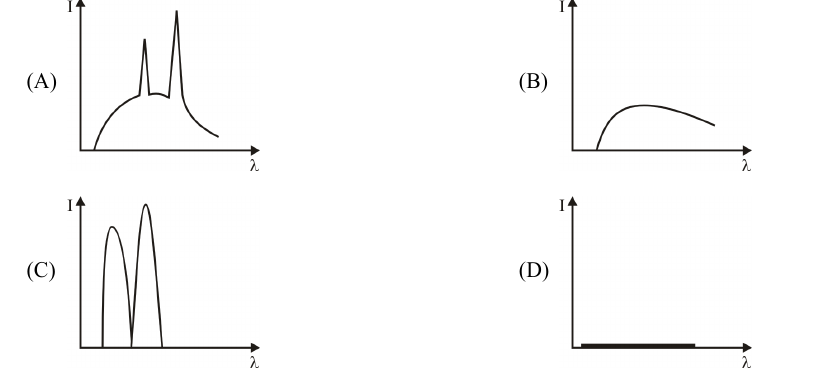
\includegraphics[width=0.62\textwidth]{Score-II - Test 36 (07 Feb 2025)-img/p1phy_q3_options.png}
\end{figure*}

\textbf{4.} A rigid ring is made to roll along the ceiling of room, where exists a uniform horizontal magnetic field of induction B perpendicular to the plane of the ring. The velocity of the centre of the ring is constant and its modulus is V. A charged particle P of mass m is fixed on the ring. The charge q on the particle is $\dfrac{kmg}{4BV}$ so that there is no force of interaction between the ring and particle. Find out value of k.

\begin{center}
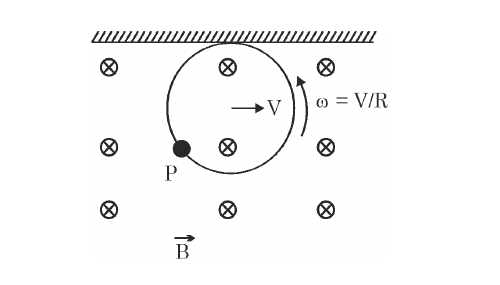
\includegraphics[width=0.9\linewidth]{Score-II - Test 36 (07 Feb 2025)-img/p1phy_q4_ring.png}
\end{center}

\begin{qoptions}
\opt{A}{4}
\opt{B}{6}
\opt{C}{1}
\opt{D}{2}
\end{qoptions}

\subsectionhdr{Section-I (ii): One or more correct}

\textbf{5.} A dielectric slab is filled in between the plates of parallel plate charged capacitor. Di-electric constant of the capacitor varies with x as $k=\dfrac xd k_0$. Capacitor is not connected with the battery. Then choose the correct statement(s).

\begin{center}
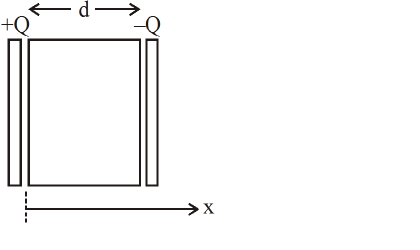
\includegraphics[width=0.75\linewidth]{Score-II - Test 36 (07 Feb 2025)-img/p1phy_q5_capacitor.png}
\end{center}

\begin{qoptions}
\opt{A}{Net electric field inside the di-electric is uniform throughout the capacitor.}
\opt{B}{Net electric field inside the dielectric decreases on moving along x-direction inside the capacitor.}
\opt{C}{Bound charge density inside the di-electric is zero.}
\opt{D}{Bound charge density inside the dielectric is non-uniform.}
\end{qoptions}

\textbf{6.} Consider the rays shown in the diagram as paraxial. The image of the virtual point object O formed by the concave lens LL' is:-

\begin{figure*}[t]
\centering
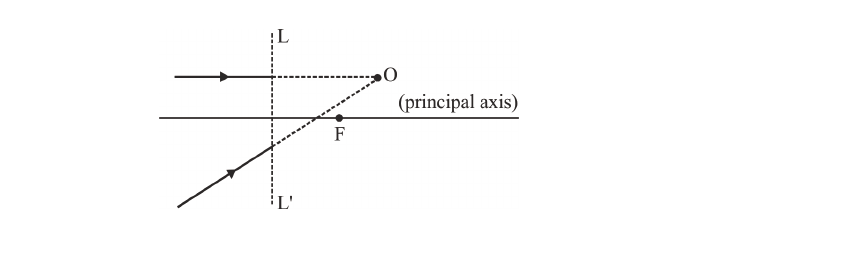
\includegraphics[width=0.55\textwidth]{Score-II - Test 36 (07 Feb 2025)-img/p1phy_q6_lens.png}
\end{figure*}

\begin{qoptions}
\opt{A}{Virtual}
\opt{B}{Real}
\opt{C}{Located below the principal axis}
\opt{D}{Located left of the lens}
\end{qoptions}

\textbf{7.} A network is given as shown. Switch was at position 1 for long time. at t = 0 it is shifted to position 2, then

\begin{center}
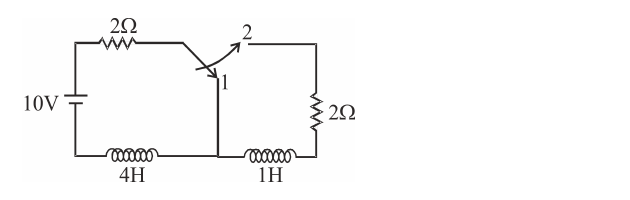
\includegraphics[width=0.95\linewidth]{Score-II - Test 36 (07 Feb 2025)-img/p1phy_q7_circuit.png}
\end{center}

\begin{qoptions}
\opt{A}{Current just after switching is $\sqrt{20}$ Amp}
\opt{B}{Current just after switching is 4 Amp}
\opt{C}{Current in the circuit varies $i=\dfrac52+\dfrac32e^{-4t/5}$}
\opt{D}{Current just after switching is 0}
\end{qoptions}

\textbf{8.} Five infinite-impedance voltmeters, calibrated to read rms values, are connected as shown in figure. Let R = 400 $\Omega$, L = 3.5 H, C = 5 $\mu$F, $\omega$ = 200 rad/s and AC voltage having rms value of 30 V. The reading of voltmeters will be:-

\begin{center}
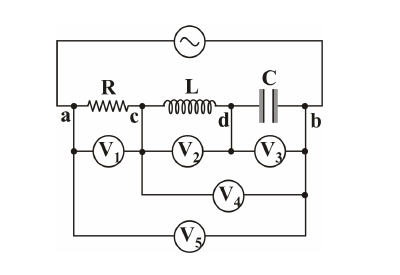
\includegraphics[width=0.85\linewidth]{Score-II - Test 36 (07 Feb 2025)-img/p1phy_q8_voltmeters.png}
\end{center}

\begin{qoptions}
\opt{A}{V$_2$ = 42 V, V$_3$ = 64 V, V$_4$ = 22 V}
\opt{B}{V$_1$ = 24 V, V$_2$ = 42 V, V$_4$ = 18 V}
\opt{C}{V$_1$ = 24 V, V$_4$ = 6 V, V$_5$ = 30 V}
\opt{D}{V$_2$ = 42 V, V$_3$ = 60 V, V$_5$ = 30 V}
\end{qoptions}

\textbf{9.} A small squirrel is put into a circular wheel cage of radius R which has a frictionless central pivot. A light horizontal platform of length 6R/5 is fixed to the wheel below the pivot as shown. Initially squirrel is at rest at one end of the platform. When the platform is released squirrel starts running but platform and wheel remain stationary. Choose the correct options.

\begin{center}
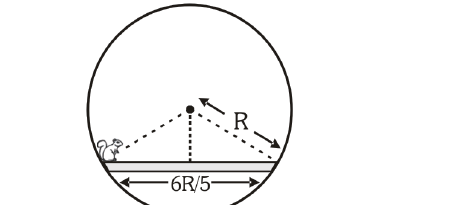
\includegraphics[width=0.8\linewidth]{Score-II - Test 36 (07 Feb 2025)-img/p1phy_q9_squirrel.png}
\end{center}

\begin{qoptions}
\opt{A}{Maximum speed of squirrel is $\sqrt{\dfrac{Rg}5}$}
\opt{B}{Maximum speed of squirrel is $\sqrt{\dfrac{9Rg}{20}}$}
\opt{C}{Maximum acceleration of squirrel is $\dfrac{4g}3$}
\opt{D}{Maximum acceleration of squirrel is $\dfrac{3g}4$}
\end{qoptions}

\textbf{10.} A gas filled tube has 2 mm inside diameter and 25 cm length. The gas is heated by an electrical wire of diameter 50 $\mu$m located along the axis of the tube. Current and voltage drop across the heating element are 0.5 A and 4 volts respectively. If the heating wire and inside of tube have temperatures 175\textdegree C and 150\textdegree C respectively, find the thermal conductivity (k) of the gas filling the tube and heat transfer rate (i). Assume mode of heat transfer as conduction only.

\begin{center}
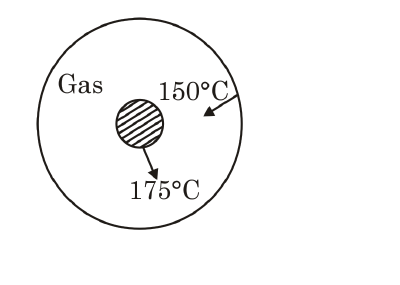
\includegraphics[width=0.65\linewidth]{Score-II - Test 36 (07 Feb 2025)-img/p1phy_q10_gastube.png}
\end{center}

\begin{qoptions}
\opt{A}{K = 0.188 W/m\textdegree C}
\opt{B}{i = 2W}
\opt{C}{k = 0.567 W/m\textdegree C}
\opt{D}{i = 6W}
\end{qoptions}

\subsectionhdr{Section-II (i): Paragraph-based Numerical}

\textbf{Paragraph for Questions 1 and 2}

Velocity of efflux in Torricelli's theorem is given by $v=\sqrt{2gh}$, here h is the height of hole from the top surface, after that, motion of liquid can be treated as projectile motion. (g = 10 m/s$^2$)

\begin{center}
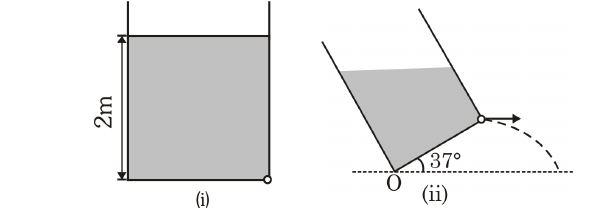
\includegraphics[width=0.95\linewidth]{Score-II - Test 36 (07 Feb 2025)-img/p1phy_n12_vessels.png}
\end{center}

\textbf{1.} Liquid is filled in a vessel of square base (2m $\times$ 2m) upto a height of 2m as shown in figure (i). In figure (ii) the vessel is tilted from horizontal at 37\textdegree. If the velocity of efflux in this case (fig. ii) is v m/s. Find value of v$^2$. (Liquid does not spills out on tilting.)

\textbf{2.} At what distance (in m) from hole, will the liquid strike on the ground? (Assume liquid comes out horizontally.)

\textbf{Paragraph for Questions 3 and 4}

A dumbell is made of two small masses B and C each of mass m, fixed by a massless rod of length L, lies on a smooth horizontal table. A ball 'A' of mass m moving with speed u = 8 m/s, strikes the ball B head on. The initial velocity of A is normal to the length of the rod. A and C collide after collision of A with B.

\begin{center}
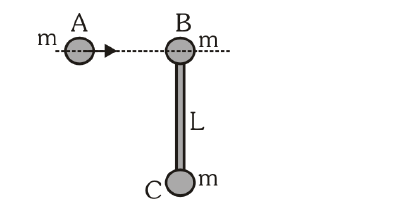
\includegraphics[width=0.55\linewidth]{Score-II - Test 36 (07 Feb 2025)-img/p1phy_n34_dumbbell.png}
\end{center}

\textbf{3.} Velocity of A just after the collision with B:-

\textbf{4.} The co-efficient of restitution is - (For collision between A and B)

\textbf{Paragraph for Questions 5 and 6}

A conducting string is rigidly clamped at the two insulated supports P and Q, separated by a distance '$L_0$'. A magnetic field of uniform intensity '$B_0$' $\otimes$ exists in the region. The string is given a slight disturbance due to which standing waves are set in and it vibrates in 5th harmonic. The maximum amplitude of oscillations of the string particles is 'A' and the angular frequency '$\omega$'. It is given that at t = 0, the particles of the string are at the mean position.

\begin{center}
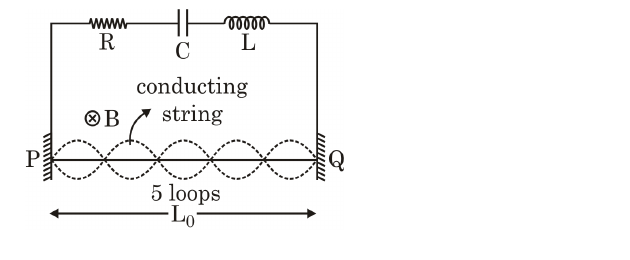
\includegraphics[width=0.95\linewidth]{Score-II - Test 36 (07 Feb 2025)-img/p1phy_n56_string.png}
\end{center}

In light of the information given above, answer the following questions.

\textbf{5.} If the maximum value of induced Electromotive force in the string is $\dfrac{\alpha B_0A\omega L_0}\pi$, then the value of $\alpha=$\_\_\_\_.

\textbf{6.} Assuming $(x_L-x_C)=\sqrt3R$, if the magnitude of current in the circuit at $t=\dfrac\pi\omega$ is $\beta\dfrac{B_0A\omega L_0}{\pi R}$, then the value of $\beta=$\_\_\_\_.

\subsectionhdr{Section-II (ii): Non-negative Integer}

\textbf{7.} The peak emission from a black body at a certain temperature occurs at a wavelength of 6000 \AA. On increasing its temperature, the total radiation emitted is increased 16 times. These radiations are allowed to fall on a metal surface. Photoelectrons emitted by the peak radiation at higher temperature can be bought to rest by applying a potential equivalent to the excitation potential corresponding to the transition for the level n = 4 to n = 2 in the Bohr's hydrogen atom. The work function of the metal is given by $\dfrac\alpha{100}$ eV where $\alpha$ is the numerical constant. Find the value of $\alpha$. [Take: hc = 12420 eV-\AA]

\textbf{8.} A conveyer belt is moving horizontally with speed 3 m/s. A small block enters the belt with velocity 4 m/s perpendicular to velocity of belt. If coefficient of friction between block and belt is 0.5, then the minimum width of belt required so that block remains on belt is (in meter)

\textbf{9.} A conducting sphere of radius '3r' having charge 'Q' is at a great distance from a neutral conducting ball of radius 'r'. They are connected with a thin perfectly conducting wire of inductance 'L' through a switch. If the maximum current in the wire after the switch is closed is $Q\sqrt{\dfrac1{k\pi\varepsilon_0rL}}$, then find the value of k.

\sectionhdr{PART-2: CHEMISTRY}
\subsectionhdr{Section-I (i): Single Correct}

\textbf{1.} Which of the following mixtures is obtained by the reaction of conc. HCl and KClO$_3$?

\begin{qoptions}
\opt{A}{O$_2$ + Cl$_2$O}
\opt{B}{O$_2$ + ClO$_2$}
\opt{C}{Cl$_2$ + ClO$_2$}
\opt{D}{Cl$_2$O + Cl$_2$}
\end{qoptions}

\textbf{2.} Incorrectly matched to their major product on treatment with sodium tert-Butoxide as base are

\begin{figure*}[t]
\centering
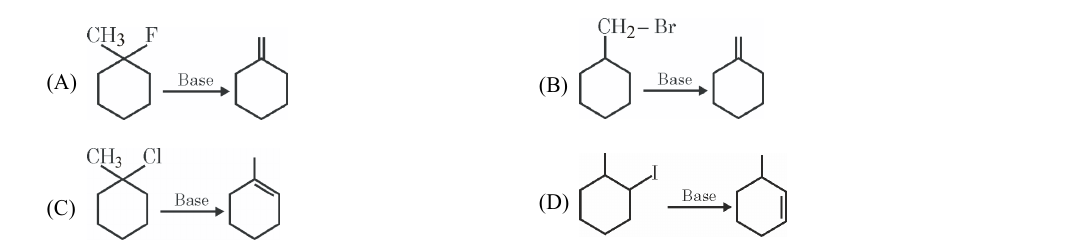
\includegraphics[width=0.85\textwidth]{Score-II - Test 36 (07 Feb 2025)-img/chem_q2_reactions.png}
\end{figure*}

\textbf{3.} 2 moles of phenol reacts with phthalic anhydride to give compound 'X'. In basic medium, compound 'X' gets converted to compound 'Y'. Degree of unsaturation in compound 'Y' is

\begin{qoptions}
\opt{A}{12}
\opt{B}{15}
\opt{C}{13}
\opt{D}{14}
\end{qoptions}

\textbf{4.} A 150 ml of solution of I$_2$ is divided into two parts. Part 1st reacts with hypo solution in acidic medium. 15 ml of 0.4 M hypo was consumed. Part 2nd was added with 100 ml of 0.3 M NaOH. Residual base required 10 ml of 0.3 M H$_2$SO$_4$ for complete neutralization. Then the incorrect statement is

\begin{qoptions}
\opt{A}{No. of moles of I$_2$ reacted in part 1st is $3\times10^{-3}$}
\opt{B}{Initial conc. of I$_2$ solution is 0.1 M}
\opt{C}{No. of moles of I$_2$ reacted in part 2nd is $15\times10^{-3}$}
\opt{D}{No. of moles of I$_2$ reacted in part 2nd is $12\times10^{-3}$}
\end{qoptions}

\subsectionhdr{Section-I (ii): One or more correct}

\textbf{5.} Consider the reaction:
\begin{center}
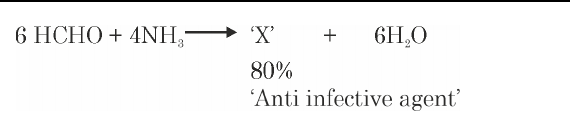
\includegraphics[width=0.9\linewidth]{Score-II - Test 36 (07 Feb 2025)-img/chem_q5_hcho.png}
\end{center}
Correct statement for 'X' is

\begin{qoptions}
\opt{A}{Maximum carbon atom present in a plane is 6}
\opt{B}{N--N bond present in X is 0}
\opt{C}{Methylene ($-$CH$_2-$) group is present in 'X' is 6.}
\opt{D}{All atoms in 'X' are sp$^3$ hybridised and total 4 lone pair is present.}
\end{qoptions}

\textbf{6.} White phosphorus on reaction with thionyl chloride PCl$_3$, SO$_2$ and a compound 'X' an analogous (same as 'X'). Compound of Se undergoes disproportionation to form Y and Z, if central atom of Y has higher oxidation state than central atom of Z, then which of the following statement is CORRECT?

\begin{qoptions}
\opt{A}{'X' has restricted rotation around single bond.}
\opt{B}{Y has 4 `90\textdegree' angle in its structure.}
\opt{C}{The oxidation state of Z is zero.}
\opt{D}{The compound Y is Se$_2$Cl$_2$}
\end{qoptions}

\textbf{7.} Consider the reaction scheme:

\begin{center}
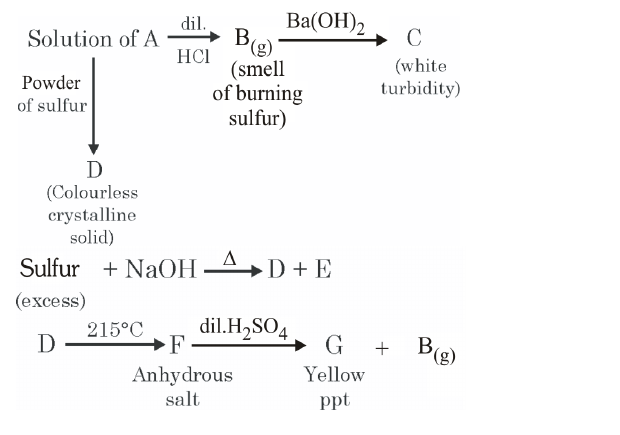
\includegraphics[width=0.85\linewidth]{Score-II - Test 36 (07 Feb 2025)-img/chem_q7_flowchart.png}
\end{center}

D is used to estimate I$_2$ quantitatively and during the reaction forms NaI and a compound H. Which of following is/are correct?

\begin{qoptions}
\opt{A}{F on reaction with Br$_2$ can produces Na$_2$SO$_4$.}
\opt{B}{F is used in photography as toner}
\opt{C}{E is Na$_2$S$_3$.}
\opt{D}{The number of water of crystallisation in D is 5.}
\end{qoptions}

\textbf{8.} In the following six electronic configuration (remaining inner orbitals are completely filled) mark the correct options.

\begin{center}
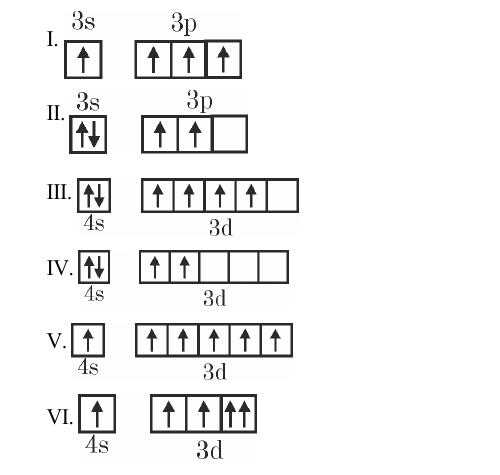
\includegraphics[width=0.75\linewidth]{Score-II - Test 36 (07 Feb 2025)-img/chem_q8_configs.png}
\end{center}

\begin{qoptions}
\opt{A}{Configuration VI violates all the three rule (Aufbau, Hund's, Pauli) rules of electronic configuration.}
\opt{B}{Spin multiplicity for V is maximum.}
\opt{C}{If configuration IV represent element X, then X$^{2+}$ ion will be diamagnetic in nature.}
\opt{D}{If configuration I represent excited state of an element Y, then it can show four covalency.}
\end{qoptions}

\textbf{9.} In a 100 ml 0.1 M CH$_3$COOH solution, 0.1 M Ca(OH)$_2$ is slowly added. Then which one of the following statement(s) is/are correct (K$_a$ of CH$_3$COOH $=10^{-5}$, log 3 = 0.5, log 2 = 0.3)

\begin{qoptions}
\opt{A}{pH of the solution will be 5 after adding 25 ml of the base.}
\opt{B}{pH of the solution will be nearly 8.9 after adding 50 ml of the base.}
\opt{C}{Before adding the base, initial pH of the solution was nearly 3.}
\opt{D}{After adding 100 ml of the base pH of the solution becomes 13.}
\end{qoptions}

\textbf{10.} Which are incorrectly matched?

\begin{qoptions}
\opt{A}{\textbf{Penicillin} : 3 chiral centre compound giving positive NaHCO$_3$ test and Lassign test give purple colour with sodium nitroprusside test.}
\opt{B}{\textbf{Azodye} : Used as antibiotic and formed when benzene diazonium ion reacts with phenol at pH = 8.5 - 9.5.}
\opt{C}{\textbf{Codeine} : Having phenolic OH and ether group and soluble in acid, with DOU = 11}
\opt{D}{\textbf{Aspirin} : It is used as nonnarcotic analgesic. It prevents blood clotting and it is formed when saliaylic acid reacts with methanol.}
\end{qoptions}

\subsectionhdr{Section-II (i): Paragraph-based Numerical}

\textbf{Paragraph for Questions 1 and 2}

Equilibrium of complex formation is of much interest for chemists. Complex formation finds potential applications in qualitative analysis, medicinal chemistry, metallurgy, electroplating etc. Theoretically the formation constant of the complex can be used to infer the stability of the complex. The overall formation constant for the reaction of CN$^-$ with Co$^{2+}$ at 298 K is $10^{19}$ and the rate constant for the formation of [Co(CN)$_6$]$^{3-}$ is $10^3$ M$^{-5}$s$^{-1}$. The standard reduction potential for the reaction [Co(CN)$_6$]$^{3-}$ + e $\to$ [Co(CN)$_6$]$^{4-}$ is $-0.835$ V. Standard reduction potential of Co$^{3+}|$Co$^{2+}$ couple is 1.82 V. $\left[\dfrac{2.303RT}F=0.059\right]$

\textbf{1.} Rate constant for the formation of [Co(CN)$_6$]$^{4-}$ is $10^X$ times greater than the rate constant for the dissociation of the same complex. Then x =

\textbf{2.} The magnitude of standard Gibbs energy change for formation of complex [Co(CN)$_6^{-4}$] (in kJ/mol) is:

\textbf{Paragraph for Questions 3 and 4}

An optically active organic compound \textbf{A} has molecular formula (C$_7$H$_{12}$O$_3$) and found to produce an yellow precipitate with alkaline solution of Iodine. Also \textbf{A} neither decolourised brown colour of bromine water nor evolved any gas with aqueous solution of NaHCO$_3$ but evolved a gas on heating with sodium metal. On hydrolysing in acidic medium, \textbf{A} produced another optically active compound \textbf{B}(C$_7$H$_{14}$O$_4$) which also produced yellow ppt with NaOH/I$_2$. Also \textbf{B} evolved a colourless, acidic gas on treatment with aqueous NaHCO$_3$ solution. \textbf{A} on treating with CrO$_3$/HCl/Pyridine in CH$_2$Cl$_2$ produced another optically active compound \textbf{C}(C$_7$H$_{10}$O$_4$). \textbf{C} on refluxing with aqueous Ag$_2$O produced an optically inactive compound \textbf{D}(C$_7$H$_{10}$O$_5$). \textbf{D} does not decarboxylate (does not evolve CO$_2$) on simple heating. However, heating \textbf{D} with sodalime gave E(C$_5$H$_{10}$O). In a separate analysis, ethyl 3-oxobutanoate was heated with excess of sodium metal and then with CH$_3$I to produce \textbf{X} (C$_8$H$_{14}$O$_3$). \textbf{X} on hydrolysis followed by simple heating of product yielded E.

\textbf{3.} Identify number of correct statements:

\begin{itemize}[leftmargin=1.6em,itemsep=1pt,topsep=2pt]
\item[(1)] 'A' gives red colour with C.A.N.
\item[(2)] Number of different functional groups in 'D' is 3
\item[(3)] 'E' gives yellow precipitate with NaOI
\item[(4)] 'C' on heating gives 2 moles CO$_2$
\item[(5)] 'B' on heating gives cyclic ester
\item[(6)] 'X' on reaction with excess D$_2$O/OD$^-$ gives product containing 5 deuterium in all the products obtained.
\end{itemize}

\textbf{4.} DOU of 'C' = P, DOU of 'A' = Q, find out $\dfrac PQ$?

\textbf{Paragraph for Questions 5 and 6}

The E$^0$ values for the changes given below are measured against SHE at 25\textdegree C.
$$\text{Cu}^{2+}+e^-\to\text{Cu}^+\quad E^0=+0.15\text{ V;}$$
$$\text{Cu}^++e\to\text{Cu},\ E^0=+0.50\text{ V;}$$
$$\text{Zn}^{2+}+2e\to\text{Zn},\ E^0=-0.76\text{ V}$$
2.303 RT/F = 0.059

\textbf{5.} The initial decrease in free energy during the cell reaction in the Galvanic cell: Zn $\left|\dfrac{\text{Zn}^{2+}}{\text{1M}}\right|\left|\dfrac{\text{Cu}^{2+}}{\text{0.1M}}\right|$ Cu is P $\times10^5$ J. The value of $|P|$ is:

\textbf{6.} The cell potential (in volts) for the cell (in volts) Zn $|$ Zn$^{+2}$(1M) $||$ Cu$^{+2}$(0.1 M) $|$ Cu is:

\subsectionhdr{Section-II (ii): Non-negative Integer}

\textbf{7.} In a FCC unit cell of 'A' atoms (At wt = 150) having side length 10\AA, the number of atom per unit cell is Z, number of next nearest neighbour is X \& packing efficiency is y \%. Find the value of $\dfrac{yz}{(x^2+1)}$. In the nearest integer.

\textbf{8.} The rate law for the reaction of OH$^-$ with tert-butyl bromide to form an elimination product in 75\% ethanol and 25\% water at 30\textdegree C in the sum of rate laws for the E$_2$ and E$_1$ reactions.
$$\resizebox{\linewidth}{!}{$r=(7.2\times10^{-5}\text{ M}^{-1}\text{S}^{-1})[\text{tert-butyl bromide}][\text{OH}^-]+(4\times10^{-5}\text{s}^{-1})[\text{tert-butyl bromide}]$}$$
What \% of reaction takes place by E$_2$ pathway, when concentration of OH$^-$ is 5 M?

\textbf{9.} Consider the reaction scheme:

\begin{center}
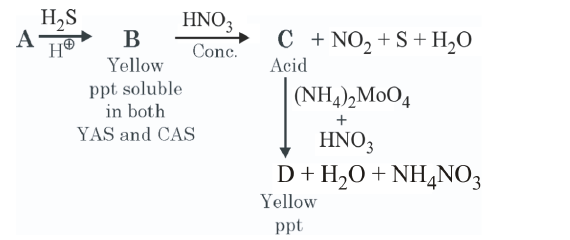
\includegraphics[width=0.75\linewidth]{Score-II - Test 36 (07 Feb 2025)-img/chem_q9_flowchart.png}
\end{center}

\begin{itemize}[leftmargin=1.6em,itemsep=1pt,topsep=2pt]
\item[(I)] D contains 'x' number of MoO$_4$ units.
\item[(II)] Atomicity in C is 'y'.
\end{itemize}

Calculate $|y-x|$

\sectionhdr{PART-3: MATHEMATICS}
\subsectionhdr{Section-I (i): Single Correct}

\textbf{1.} If $x,y,z>0$ and $x+y+z=1$, then least value of the expression $\left(\dfrac{4x+2}{2-x}+\dfrac{4y+2}{2-y}+\dfrac{4z+2}{2-z}\right)$ is

\begin{qoptions}
\opt{A}{4}
\opt{B}{5}
\opt{C}{6}
\opt{D}{7}
\end{qoptions}

\textbf{2.} If $\sin x+\sin y\geq\cos\alpha\cdot\cos x,\ \forall x\in\mathbb R$, then $\sin y+\cos\alpha$ is equal to

\begin{qoptions}
\opt{A}{$-2$}
\opt{B}{$-\dfrac32$}
\opt{C}{0}
\opt{D}{1}
\end{qoptions}

\textbf{3.} If $xf(x)=3(f(x))^2+2$, then $\displaystyle\int\dfrac{2x^2-12x\cdot f(x)+f(x)^2}{(6f(x)-x)(x^2-f(x))}\,dx$ (Where 'c' is the constant of integration)

\begin{qoptions}
\opt{A}{$\dfrac1{x^2-f(x)}+c$}
\opt{B}{$\dfrac{-1}{x^2-f(x)}+c$}
\opt{C}{$\dfrac1{(6f(x)-x)(x^2-f(x))}+c$}
\opt{D}{$\dfrac{-1}{(6f(x)-x)(x^2-f(x))}+c$}
\end{qoptions}

\textbf{4.} For positive t; let $\alpha$ and $\beta$ be the roots of $x^2+t^2x-2t=0$. If minimum value of $\displaystyle\int_{-1}^2\left(\left(x+\dfrac1{\alpha}\right)\left(x+\dfrac1\beta\right)+\dfrac1{\alpha\beta}\right)dx$ is $p+\sqrt q$, where $p\in$ Rational number and $q\in$ Natural number, then value of $[p]+q$ is (where $[\,.\,]$ denotes greatest integer function)

\begin{qoptions}
\opt{A}{1}
\opt{B}{2}
\opt{C}{3}
\opt{D}{4}
\end{qoptions}

\subsectionhdr{Section-I (ii): One or more correct}

\textbf{5.} Let $P\equiv\left(\dfrac1{\sqrt2},\dfrac1{\sqrt2}\right)$; $Q\equiv\left(-\dfrac1{\sqrt2},-\dfrac1{\sqrt2}\right)$ be the vertices of regular polygon having 12 sides such that PQ is a diameter of the circle circumscribing the polygon. Which of the following points can be the vertex of this polygon

\begin{qoptions}
\opt{A}{$\left(\dfrac{\sqrt3-1}{2\sqrt2},\dfrac{\sqrt3+1}{2\sqrt2}\right)$}
\opt{B}{$\left(\dfrac{\sqrt3+1}{2\sqrt2},\dfrac{\sqrt3-1}{2\sqrt2}\right)$}
\opt{C}{$\left(\dfrac{\sqrt3+1}{2\sqrt2},\dfrac{1-\sqrt3}{2\sqrt2}\right)$}
\opt{D}{$\left(-\dfrac12,\dfrac{\sqrt3}2\right)$}
\end{qoptions}

\textbf{6.} Let $P(x)=x^3+ax^2+bx+c$ be a polynomial, where $a,b,c\in I$ and c is an odd integer. Let $P_i$ be the value of $P(x)$ at $x=i$, given that $P_1^3+P_2^3+P_3^3=3P_1P_2P_3$. then (Where I is the set of integers)

\begin{qoptions}
\opt{A}{$P(x)$ is increases in $(3,\infty)$}
\opt{B}{$P(x)$ is decreases in $(-1,2)$}
\opt{C}{$P(x)$ can't have local maxima or local minima.}
\opt{D}{$P(x)$ has local maxima and local minima}
\end{qoptions}

\textbf{7.} Let $f:\mathbb R-\left\{-\dfrac12\right\}\to\mathbb R$ be defined by $f(x)=\dfrac{4x^2+12x+3}{4x^2+4x+1}$. Then which of the following options is (are) TRUE?

\begin{qoptions}
\opt{A}{$f(x)$ is onto function.}
\opt{B}{If $A=\left\{a:\dfrac{4x^2+12x+3}{4x^2+4x+1}=a\text{ has two solution}\right\}$ then the set $A\cap\mathbb N$ has at least 3 elements. ($\mathbb N$ is set of natural numbers)}
\opt{C}{If $B=\left\{b:\dfrac{4x^2+12x+3}{4x^2+4x+1}=b\text{ has one solution}\right\}$ then $|B|\geq2$.}
\opt{D}{$f(x)$ is decreasing in the interval $(-\infty,-1]$}
\end{qoptions}

\textbf{8.} If $a_1=1$ and for $n>1$, $a_n=a_{n-1}+\dfrac1{a_{n-1}}$ then $\left[\sin^{-1}(a_{75}-12)\right]$ can't be equal to where $[\ ]$ is greatest integer function

\begin{qoptions}
\opt{A}{$-2$}
\opt{B}{$-1$}
\opt{C}{2}
\opt{D}{$-3$}
\end{qoptions}

\textbf{9.} The value of $\displaystyle\sum_{0\leq p\leq q\leq r<s=t\leq n}1$

\begin{qoptions}
\opt{A}{$^{n+1}C_4+2\,^{n+1}C_3+\,^{n+1}C_2$}
\opt{B}{$^{n+3}C_4$}
\opt{C}{$^{n+1}C_5+2\,^{n+1}C_4+\,^{n+1}C_3$}
\opt{D}{$^{n+3}C_5$}
\end{qoptions}

\textbf{10.} Given that $\cot x=a_0x^{-1}+a_1x+a_2x^3+\ldots+a_kx^{2k-1}+\ldots\infty$ terms $\forall\ 0<|x|<\pi$, then which of the following are correct?

\begin{qoptions}
\opt{A}{$a_0=1$}
\opt{B}{$a_0=3|a_1|$}
\opt{C}{$a_0+a_1=\dfrac43$}
\opt{D}{$a_0+9a_1^2=2$}
\end{qoptions}

\subsectionhdr{Section-II (i): Paragraph-based Numerical}

\textbf{Paragraph for Questions 1 and 2}

If $f(x)$ is twice differentiable function wherever it is continuous and $f'(c_1)=f'(c_2)=0$. $f''(c_1)\cdot f''(c_2)<0$, $f(c_1)=5$, $f(c_2)=0$ and $(c_1<c_2)$.

\textbf{1.} If $f(x)$ is continuous in $[c_1,c_2]$ and $f''(c_1)-f''(c_2)>0$, then minimum number of solution of $f'(x)=0$ in $[c_1-1,c_2+1]$ is

\textbf{2.} If $f(x)$ is continuous in $[c_1,c_2]$ and $f''(c_1)-f''(c_2)<0$, then minimum number of solution of $f'(x)=0$ in $[c_1-1,c_2+1]$ is

\textbf{Paragraph for Questions 3 and 4}

Let a function is defined by $f:\mathbb R-\{0\}\to\mathbb R-\{0\}$. A line $\dfrac x{-2}=\dfrac{f(t)}t=t^2z$ is perpendicular to the line of intersection of the planes
$$P_1: tf(t)x+f\left(\dfrac1{t^2}\right)z+f(-t)=0$$
$$P_2: ty+f(-t)z+f(t^2)=0$$

\textbf{3.} Let $t=\tan\theta$ where $\theta\in\mathbb R-\left\{(2n+1)\dfrac\pi2,\dfrac{n\pi}4,n\pi\pm\dfrac\pi4\right\}$, where n is integer such that $f(\tan\theta)+\tan(\lambda\theta)f\left(\cot^2\theta\right)=0$. Then $\dfrac1{2\lambda}$ is equal to (Where $\lambda\in\mathbb N$)

\textbf{4.} Let $f(t)$ is an identity function in the domain. If a plane is obtained by rotating $P_2$ about its line of intersection with $P_1$ by 90\textdegree\ and this new plane passes through origin then sum of all values of t is equal to

\textbf{Paragraph for Questions 5 and 6}

If the area bounded by the function $f(x)=\cos^{-1}(\cos x)^2$ and $g(x)=\left(\cos^{-1}(\cos(x))\right)^2$ and $x=\pm2\pi$ is equal to $\dfrac{a(\pi^3+1)-b\pi^2}c$, where $a,b,c\in\mathbb N$, where a \& c are co-prime.

\textbf{5.} The value of $\dfrac1{12}\left(a+\dfrac bc\right)$ is

\textbf{6.} Three dice are thrown simultaneously and p is the probability that sum of numbers appearing on each of the three dice is divisible by $a+b+c$. Then $36p$ is equal to

\subsectionhdr{Section-II (ii): Non-negative Integer}

\textbf{7.} The number of the roots $\omega$ of the equation $\omega^{2025}=1$ such that $|\omega+1|\geq\sqrt{2+\sqrt2}$ are

\textbf{8.} Let $\alpha$ and $\beta$ ($\alpha<\beta$) are the solution of the equation, $x^9-81x-62=18x^3(3x+2)^{1/3}$. If
$$A=\begin{bmatrix}-\alpha&\beta+1&1\\0&\beta&2\\0&0&|\alpha|\end{bmatrix};\quad B=\begin{bmatrix}-\alpha&1&\beta\\1&\beta+1&4\\1&-\alpha&3\end{bmatrix},$$
then the value of $|\text{adj}(\text{adj}(-\alpha A))|+|\text{adj}(B)^\beta|$ is equal to.

\textbf{9.} The number of permutations x$_1$, x$_2$, x$_3$, x$_4$, x$_5$ of numbers 1, 2, 3, 4, 5 taken all at a time such that $(x_1x_2x_3+x_2x_3x_4+x_3x_4x_5+x_4x_5x_1+x_5x_1x_2)$ is divisible by 3 is

\end{document}
